\section{Umsetzung}
%was für komponenten braucht, etwas was auffinden ermöglicht, etwas was als server fungiert, jeder client ist server und client, wie finde ich server
%Erst erklären was ich machen: wie hab ich es gemacht. Hier auch diagramme einfügen 
%Um einen funktionierenden Chatroom zu bauen, werden verschiedene Komponenten für unterschiedliche Aufgaben benötigt. 
Die Applikation soll es ermöglichen, dass mehrere Nutzer im selben Netzwerk miteinander chatten können. 
Dafür müssen zu Beginn andere Teilnehmer im Netzwerk gefunden werden.
Da kein Server angefragt werden kann, um herauszufinden welche Teilnehmer es gibt, müssen sich die Geräte untereinander finden. Mithilfe eines Multicasts könnte ein neuer User 
herausfinden, wer bereits im Chatroom und im Netzwerk vorhanden ist. 
Wurde ein Chatteilnehmer gefunden, muss sowohl die Adresse als auch der Name des jeweils anderen herausgefunden und gespeichert werden. 
Mit einer angelegten Liste könnte die Speicherung der User vorgenommen werden. Somit weiß jeder Nutzer welche anderen Teilnehmer vorhanden sind. 

Nach dem Beitritt können Nachrichten verschickt werden. 
Gleichzeitig muss es neben dem Schreiben von Nachrichten möglich sein andere Nachrichten zu empfangen. 
Multithreading wäre eine Lösung um einerseits dauerhaft auf eine Eingabe des Users zu warten und andererseits die Api zu starten um gesendeten Nachrichten der Anderen zu empfangen.
Jeder User kann alle gesendeten Nachrichten lesen, da es sich um einen großen Chatroom handelt. 
Damit jeder Teilnehemr die gesendete Nachricht erhält, muss sie an jede vorhandene Adresse in der Liste verschickt werden.

Möchte ein User den Chatroom verlassen, muss sichergestellt werden, dass dieser nach dem Austritt keine weiteren Nachrichten erhält. 
Mit dem Verlassen des Chatrooms müssen die anderen Geräte informiert werden, dass diese Adresse nicht mehr vorhanden ist und keine weiteren Nachrichten zugestellt werden.
Durch das Versenden einer speziellen Nachricht beim Verlassen mit den eigenen Daten kann der Teilnehmer aus der Liste der anderen User gelöscht werden. 
Die Chat Applikation ist damit beendet. 
\\
\subsection{Ablauf}
Beim Starten der Chat-Anwendung findet eine Initialisierung statt. 
Der Client soll mithilfe eines mdns Broadcast andere Chatteilnehmer finden.
Wurde ein anderer Teilnehmer gefunden bekommt der Client eine mdns Antwort mit der IP Adresse des Teilnehmers.
Die IP Adresse wird von dem DiscoveryService in eine Userliste eingetragen. 
An jede gefundene IP Adresse wird eine Startmessage mit eigener IP Adresse und Name über HTTP geschickt. Der andere Teilnehmer kann somit den neuen 
User in seiner Liste ergänzen und ebenfalls eine Startmessage mit seinem Namen als Antwort schicken. Der neue Client ergänzt in seiner Userliste 
den Namen. Damit ist die Initialisierung abgeschlossen. 
\begin{figure}[h]
    \centering
    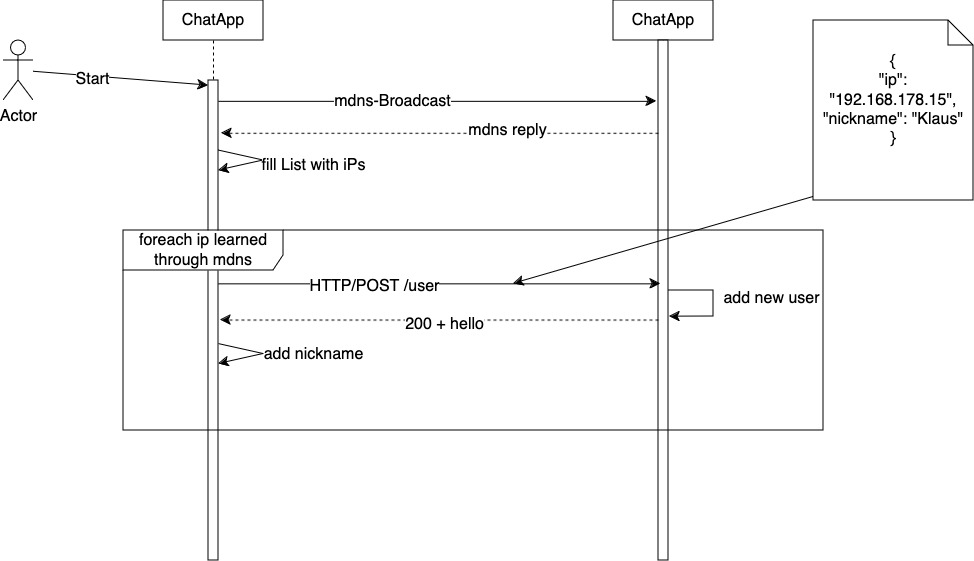
\includegraphics[scale=0.4]{Images/Initialisierung_Sequenzdiagramm.jpg}
    \captionbelow{Initialisierung}
\end{figure}
\newpage
Nachdem man dem Chatroom beigetreten ist können Nachrichten verschickt werden. Der User schreibt eine Nachricht. 
Um diese Nachricht zu verschicken muss der Client in der Userliste alle IP Adressen der Teilnehmer nachschauen. Die Nachricht wird anschließend 
an jede einzelne IP Adresse geschickt. Das Versenden der Nachrichten findet ebenfalls mittels HTTP statt.
\begin{figure}[ht]
    \centering
    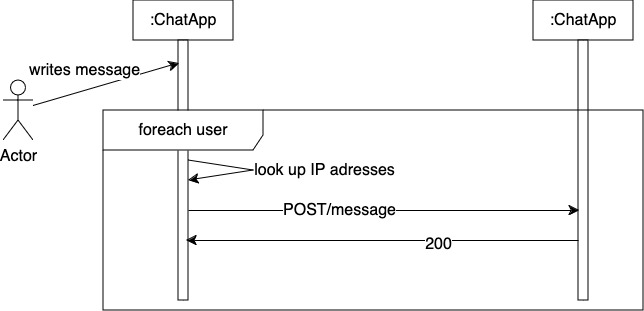
\includegraphics[scale=0.4]{Images/Conversation_Sequenzdiagramm.jpg}
    \captionbelow{Kommunikation}
\end{figure}
\\
Um den Chatroom zu verlassen wird wieder über HTTP eine Exitmessage an alle Teilnehmer gesendet. Die Exitmessage enthält wie die Startmessage den eigenen Namen und IP Adresse.
Der User wird von den anderen Teilnehmern aus der Userliste entfernt und der Client ist somit dem Chatroom ausgetreten. 
\begin{figure}[ht]
    \centering
    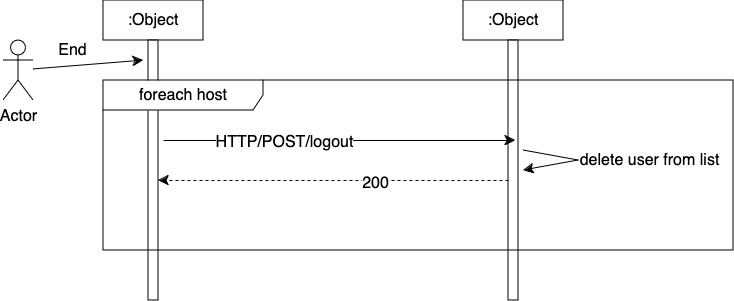
\includegraphics[scale=0.4]{Images/Exit_Sequenzdiagramm.jpg}
    \captionbelow{Exit}
\end{figure}
\newpage
\subsection{Aufbau und Komponenten} %woraus die sachen bestehen 
Der Chat client setzt sich im wesentlichen zusammen aus:
\begin{itemize}
    \item DiscoveryService
    \item Receiver
    \item Transmitter
    \item ConfigData
    \item Message types
\end{itemize} 
Um mit dem chatten starten zu können wird der DiscoveryService benötigt. 
Er ist für den Multicast und das Eintragen der Teilnehmer in die Userliste verantwortlich. Zudem sorgt er dafür, dass der Computer im Netzwerk weiterhin zu finden ist für andere User.
Der Receiver ist für das Empfangen der Startmessage, der normalen Nachrichten und der Exitmessage zuständig. Des Weiteren wird die API gestartet und die verschiedenen Endpunkte festgelget.
Der Transmitter übernimmt die Funktion des Sendens der Messages und der ExitMessage. 
Für das Empfangen, Versenden und Suchen von Teilnehmern sind mehrere Abläufe gelichzeitig nötig. Hierbei werden Threads verwendet um zeitgleich verschiedene Prozesse laufen zu lassen.
In der ConfigData ist die Userliste mit IP Adresse und Name der User angelegt und die eigenen Daten.
Die Message types definieren die einzelnen Typen und den Aufbau der unterschiedlichen Messagearten. Diese unterteilen sich in StartMessage, Message und ExitMessage.
Um Nachrichten zu versenden werden HTTP requests und eine REST API verwendet. 

\subsection{Ausführung}
\subsubsection{Start}
Mit dem Start der Applikation wird zuerst der Name des Benutzers mit einer Eingabe festgelegt. Danach wird der Receiver gestartet. Er sorgt dafür, dass sowohl Startmessages, normale Messages als auch Exitmessages empfangen werden können. Außerdem wird mit dem Receiverstart die API gestartet.
Anschließend beginnt der DiscoveryService mit einem Multicast nach anderen Teilnehmern zu suchen. Es muss sichergestellt werden, dass in einem bestimmten, vorher definierten Netz gesucht wird,
um sich mit anderen Teilnehmern im selben Netzwerk zu verbinden. Das Netzwerk wird mit dem Port, dem Servernamen und der IP Adresse festgelegt. Es wird definiert, wie lange nach anderen Usern im Netzwerk gesucht werden soll, bevor an die gefundenen
Teilnehmer eine StartMessage rausgeht. Die gefundenen IP Adressen werden in eine Liste eingetragen. 
Nach Ablauf der Zeit wird eine StartMessage an alle eingetragenen Adressen der Liste geschickt. Diese enthält den eigenen Namen und die IP Adresse. 
Als Antwort auf die StartMessage wird ebenfalls eine Startmessage mit Name und IP Adresse des gefundenne Users zurückgegeben.
Der Name wird passend zur IP Adresse ergänzt und die Liste in der ConfigData verwaltet. 
Der DiscoveryService bleibt auch nach Beendigung der Suche weiterhin aktiv um auf eingehende Startmessages von weiteren Teilnehmern antworten zu können und diejenigen in der Userliste zu ergänzen.

%Die MyListener Klasse sucht mit der Methode add\_service nach IP Adressen im Netzwerk. Mithilfe der Zeroconf library können die Adressen im angegebenen Netzwerk gefunden werden.
%Hier beschränkt sich die Suche auf das Netzwerk \_airplay.\_tcp.local. Die gefundenen Adressen werden der Liste \_userlist hinzugefügt. 
%Die Userliste befindet sich in der ConfigData. Die ConfigData besteht aus den eigenen Daten, IP Adresse und Name, und der Userliste. 
%Der eigene Name wird beim Programmstart eingegeben. 
%In der Liste befinden sich die gefundenen IP Adressen mit den dazugehörigen Namen.
%Blabla greift auf userliste zu und trägt ein\dots
%Nach der Teilnehmersuche schickt der DiscoverService an jede gefundene Adresse eine StartMessage. In der StartMessage befindet sich die eigene IP Adresse und der Name.
%Um die eigene IP Adresse herauszufinden wird die netifaces library in der ConfigData verwendet und als IPv4Adresse gespeichert. 
%Der DiscoveryService ruft die Userliste auf und sendet über HTTP an jede eingetragene Adresse eine Startmessage an den Endpunkt start.

\subsubsection{Messages}
Nach Abschluss der Initialisierung und dem Beitritt zum Chatroom können Nachrichten verschickt werden. Durch den Start des Transmitters wird durchgehend eine Nachrichteneingabe des Nutzers gefordert, 
bis das Wort \emph{exit} eingegeben wird.
Die eingegebene Nachricht wird an alle anderen Teilnehemer gesendet. Dafür muss die Nachricht an jede einzelne IP Adresse, die in der Userliste vorhanden ist, geschickt werden.
Eingehende Nachrichten werden vom Receiver empfangen und mit dem Namen des Senders auf die Konsole gedruckt. 

%Nach Abschluss der Initialisierung und dem Beitritt zum Chatroom, sorgt der Transmitter für die Nachrichteneingabe. 
%Es wird dauerhaft eine Eingabe vom User gefordert.
%Der Transmitter geht die Userliste durch und sendet an jede Adresse die Nachricht an den Endpunkt message.
%Das Beenden der Eingabe und der Austritt aus dem Chatroom findet erst statt, wenn "'exit"' eingeben wird.
%Die while Schleife sorgt dafür, dass so lange eine Eingabe gefordert wird, bis "'exit"' eingegeben wird.  
%Gleichzeitig werden Nachrichten empfangen. Im Receiver sind Methoden definiert um die Startmessage, Message und Exitmessage zu erhalten.
%Mit dem Import von FastAPI kann das Abrufen und Senden an definierte Endpunkte stattfinden. 
%Es werden in der \_\_init\_\_ Funktion des Receivers die Routen zu den jeweiligen Endpunkten start, message und exit mit den dazugehörigen Funktionen angegeben.
%Die Methode receive\_start\_message fordert eine Nachricht vom Typ StartMessage und trägt die übergebenen Variablen innerhalb der Startmessage, name und ip, in die userliste der ConfigData ein.
%Receive\_message fordert einen Parameter vom Typ Message und gibt diesen in der Konsole aus.
%Um die Exitmessage zu empfangen gibt es die Methode receive\_exit\_message. Hier wird eine Nachricht vom Typ ExitMessage übergeben und die darin enthaltene IP Adresse wird aus der user\_list entfernt.
%Neben dem Empfangen von Nachrichten startet der Receiver mit der Methode run\_api die API. Dabei werden Host und Port übergeben, wobei der Host die eigene IP Adresse ist.
\subsubsection{Exit}
Um das Programm zu beenden gibt der User in die Konsole \emph{exit} ein. Dadurch wird die andauernde Forderung einer Nachrichteneingabe beendet.
Der DiscoveryService stoppt das Advertisement, damit man für andere User nicht mehr zu finden ist. Nachfolgend sendet der Transmitter eine Exitmessage 
an alle gespeicherten Adressen in der UserListe. Die geschickte IP Adresse mit der Exitmessage wird von den anderen Usern aus der Liste gelöscht. 
Somit werden keine weiteren Nachrichten mehr an einen zugestellt. Nach der Exitmessage wird der Receiver gestoppt um die API zu stoppen. 
Schlussendlich wird der Thread geschlossen und das Programm ist beendet. 